\documentclass{article}
\usepackage[utf8]{inputenc}
\usepackage[T1]{fontenc}
\usepackage[spanish, es-tabla]{babel}
\usepackage{graphicx} % Paquete fundamental para insertar imágenes
\usepackage{caption}  % Para personalizar el epígrafe
\usepackage[legalpaper, margin=2cm]{geometry} 

% Configuración del estilo de epígrafe tipo tesina
\captionsetup[figure]{
    labelfont=bf,      % "Figura X" en negrita
    textfont=it,        % El título en cursiva
    labelseparator=period, % Punto después del número (Figura 1.)
    justification=centering % Centrado
}

\begin{document}

% Si quieres forzar el número de la imagen manualmente, por ejemplo a "Figura 5"
% \setcounter{figure}{4} 

%  RADIOS DATASETS
% Radio Shuttle todas las clases
\begin{figure}[ht]
    \centering
    % Reemplaza 'nombre_de_tu_archivo' por el nombre de tu imagen (ej. 'grafico_f1.png')
    % El [width=0.8\textwidth] escala la imagen al 80% del ancho del texto
    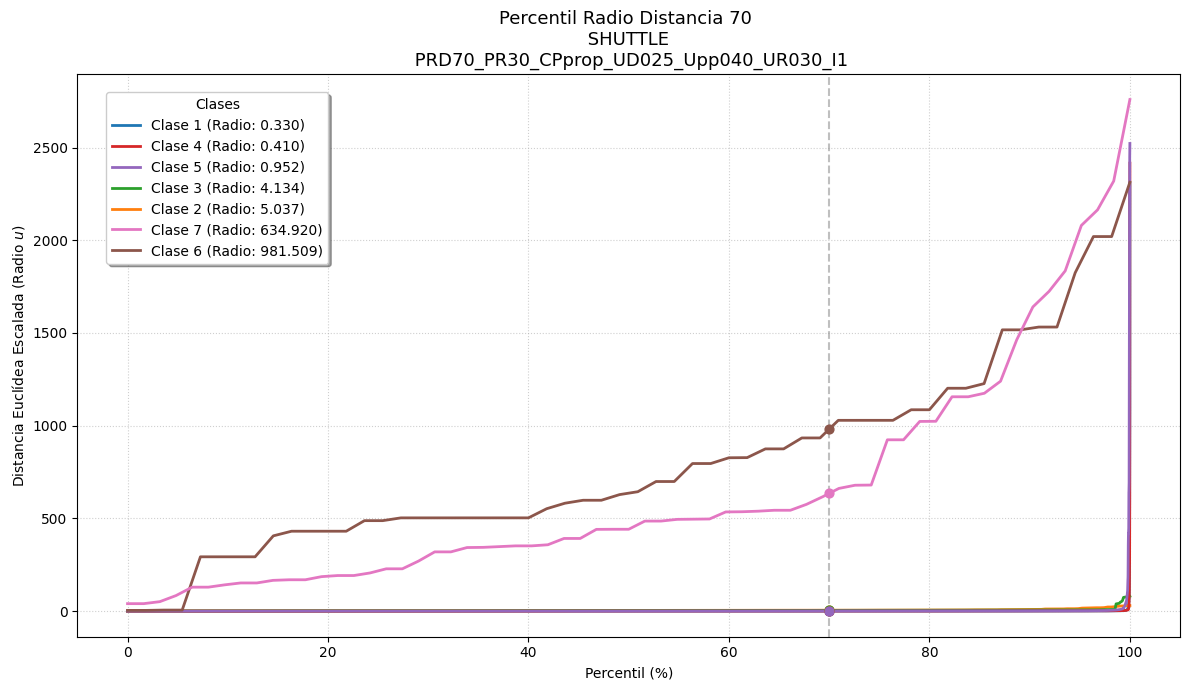
\includegraphics[width=1\textwidth]{radios/shuttle-1_radio.png}
    
    % El epígrafe (caption)
    \caption{Visualizacion de radios por clase del dataset Shuttle.}
    \label{fig:mi_grafico_1}
\end{figure}

% Radio Shuttle clases 1 a 5
\begin{figure}[ht]
    \centering
    % Reemplaza 'nombre_de_tu_archivo' por el nombre de tu imagen (ej. 'grafico_f1.png')
    % El [width=0.8\textwidth] escala la imagen al 80% del ancho del texto
    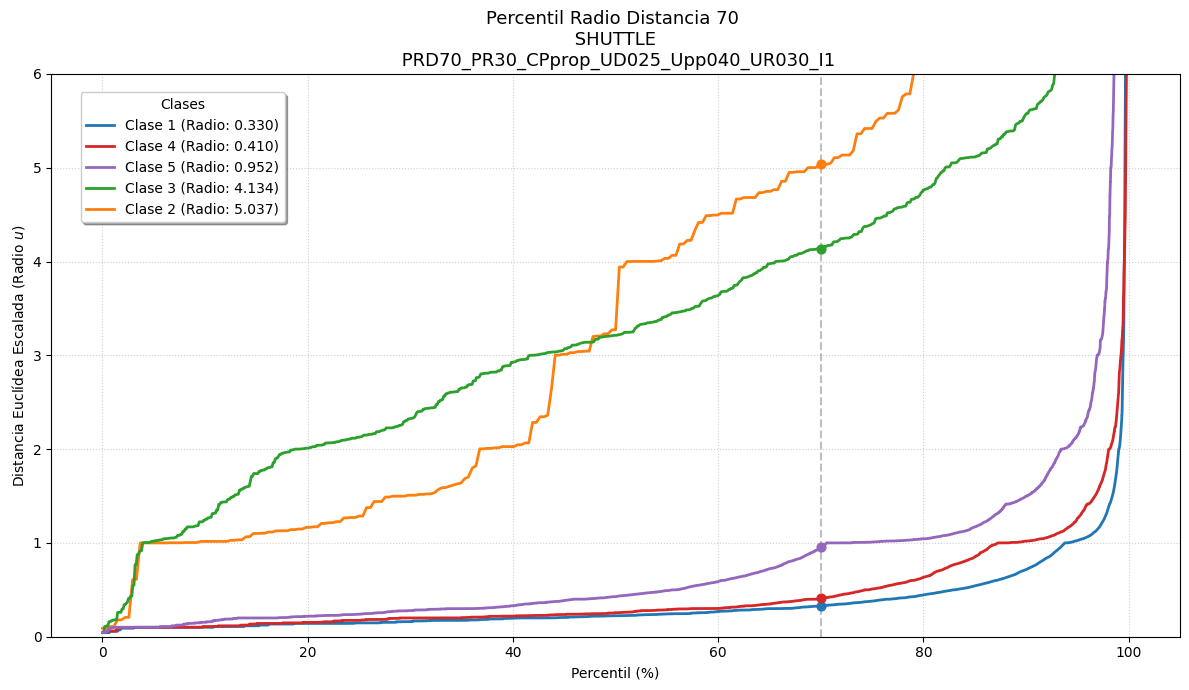
\includegraphics[width=1\textwidth]{radios/shuttle-2_radio.png}
    
    % El epígrafe (caption)
    \caption{Visualizacion de radios con foco en las clases 1 a 5 del dataset Shuttle.}
    \label{fig:mi_grafico_2}
\end{figure}


% Radio telco_churn todas las clases
\begin{figure}[ht]
    \centering
    % Reemplaza 'nombre_de_tu_archivo' por el nombre de tu imagen (ej. 'grafico_f1.png')
    % El [width=0.8\textwidth] escala la imagen al 80% del ancho del texto
    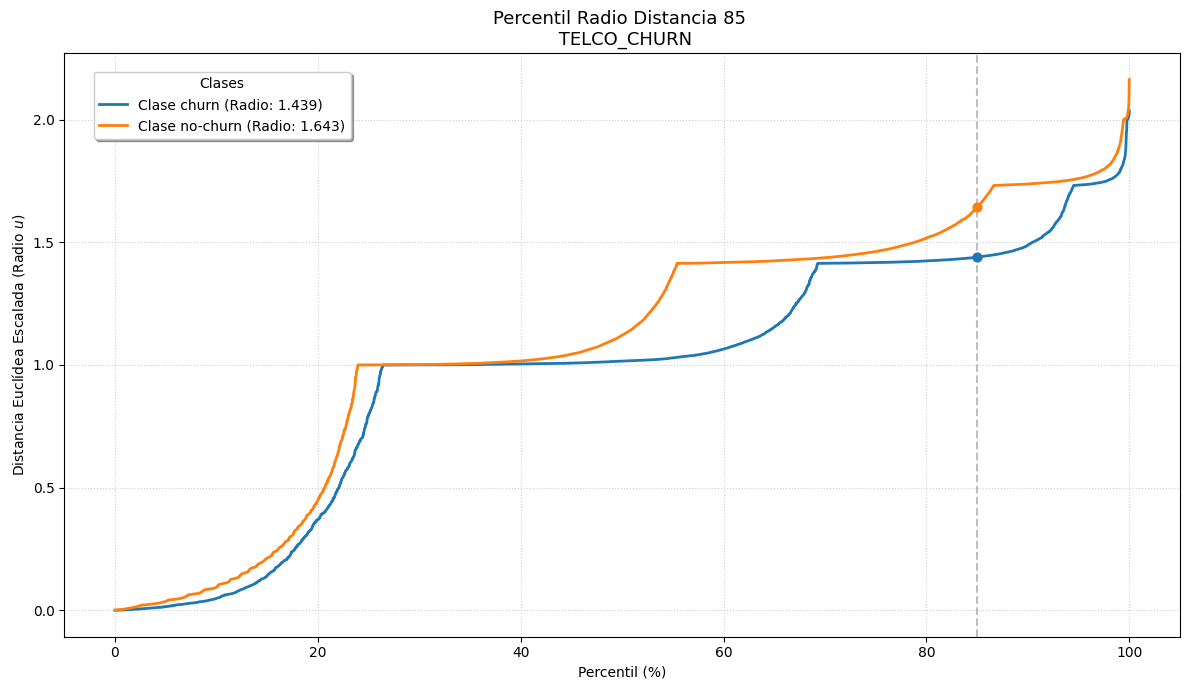
\includegraphics[width=1\textwidth]{radios/telco_churn_radio.png}
    
    % El epígrafe (caption)
    \caption{Visualizacion de radios por clase del dataset Telco Churn.}
    \label{fig:mi_grafico_3}
\end{figure}

% Radio us_crime todas las clases
\begin{figure}[ht]
    \centering
    % Reemplaza 'nombre_de_tu_archivo' por el nombre de tu imagen (ej. 'grafico_f1.png')
    % El [width=0.8\textwidth] escala la imagen al 80% del ancho del texto
    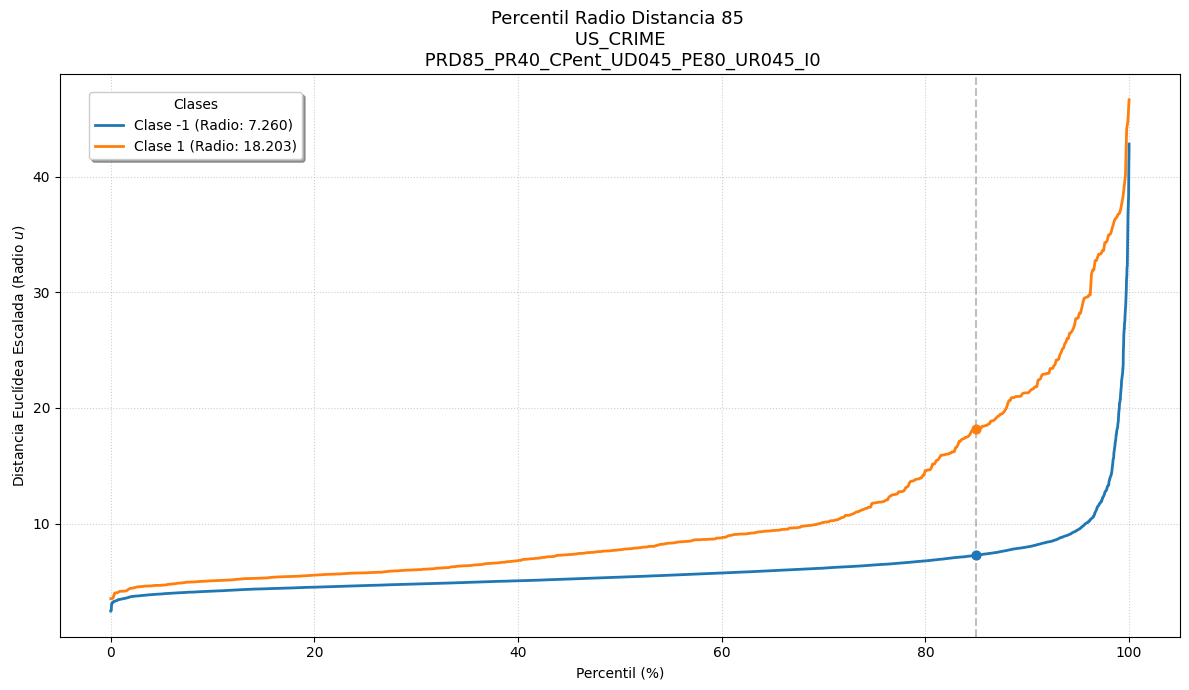
\includegraphics[width=1\textwidth]{radios/us_crime_radio.png}
    
    % El epígrafe (caption)
    \caption{Visualizacion de radios por clase del dataset US Crime.}
    \label{fig:mi_grafico_4}
\end{figure}

% Radio predict_faults todas las clases
\begin{figure}[ht]
    \centering
    % Reemplaza 'nombre_de_tu_archivo' por el nombre de tu imagen (ej. 'grafico_f1.png')
    % El [width=0.8\textwidth] escala la imagen al 80% del ancho del texto
    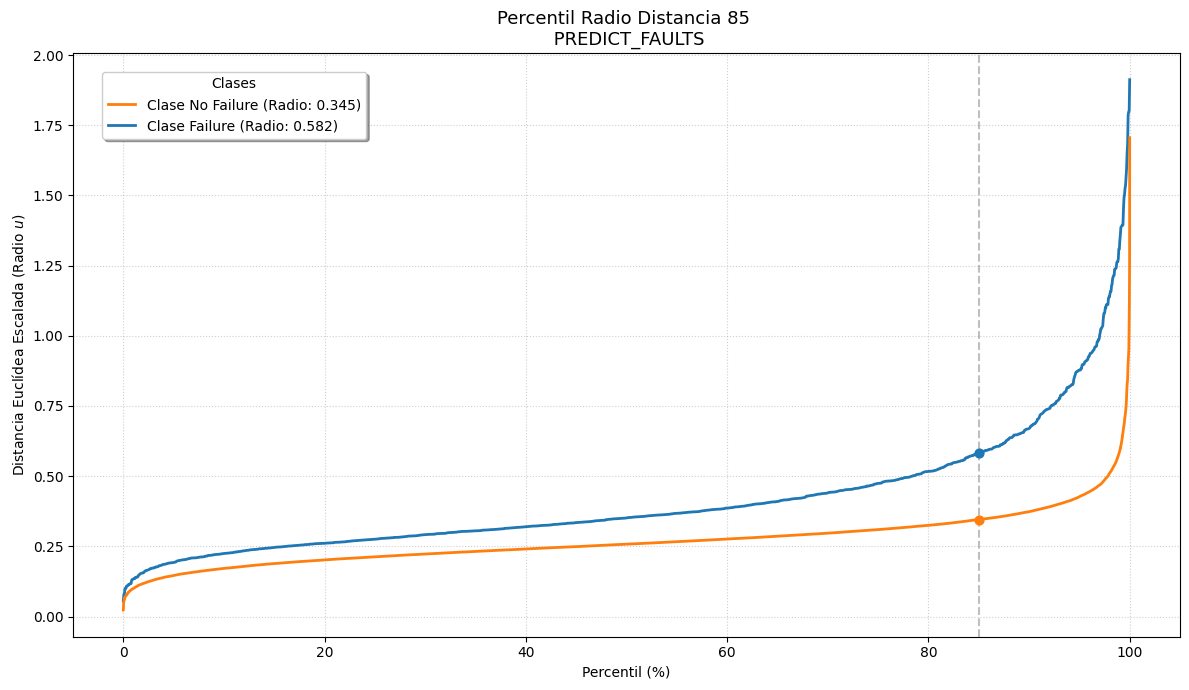
\includegraphics[width=1\textwidth]{radios/predict_faults_radio.png}
    
    % El epígrafe (caption)
    \caption{Visualizacion de radios por clase del dataset Predict Faults.}
    \label{fig:mi_grafico_5}
\end{figure}

%  PUREZAS DATASETS 

% Pureza Shuttle todas las clases
\begin{figure}[ht]
    \centering
    % Reemplaza 'nombre_de_tu_archivo' por el nombre de tu imagen (ej. 'grafico_f1.png')
    % El [width=0.8\textwidth] escala la imagen al 80% del ancho del texto
    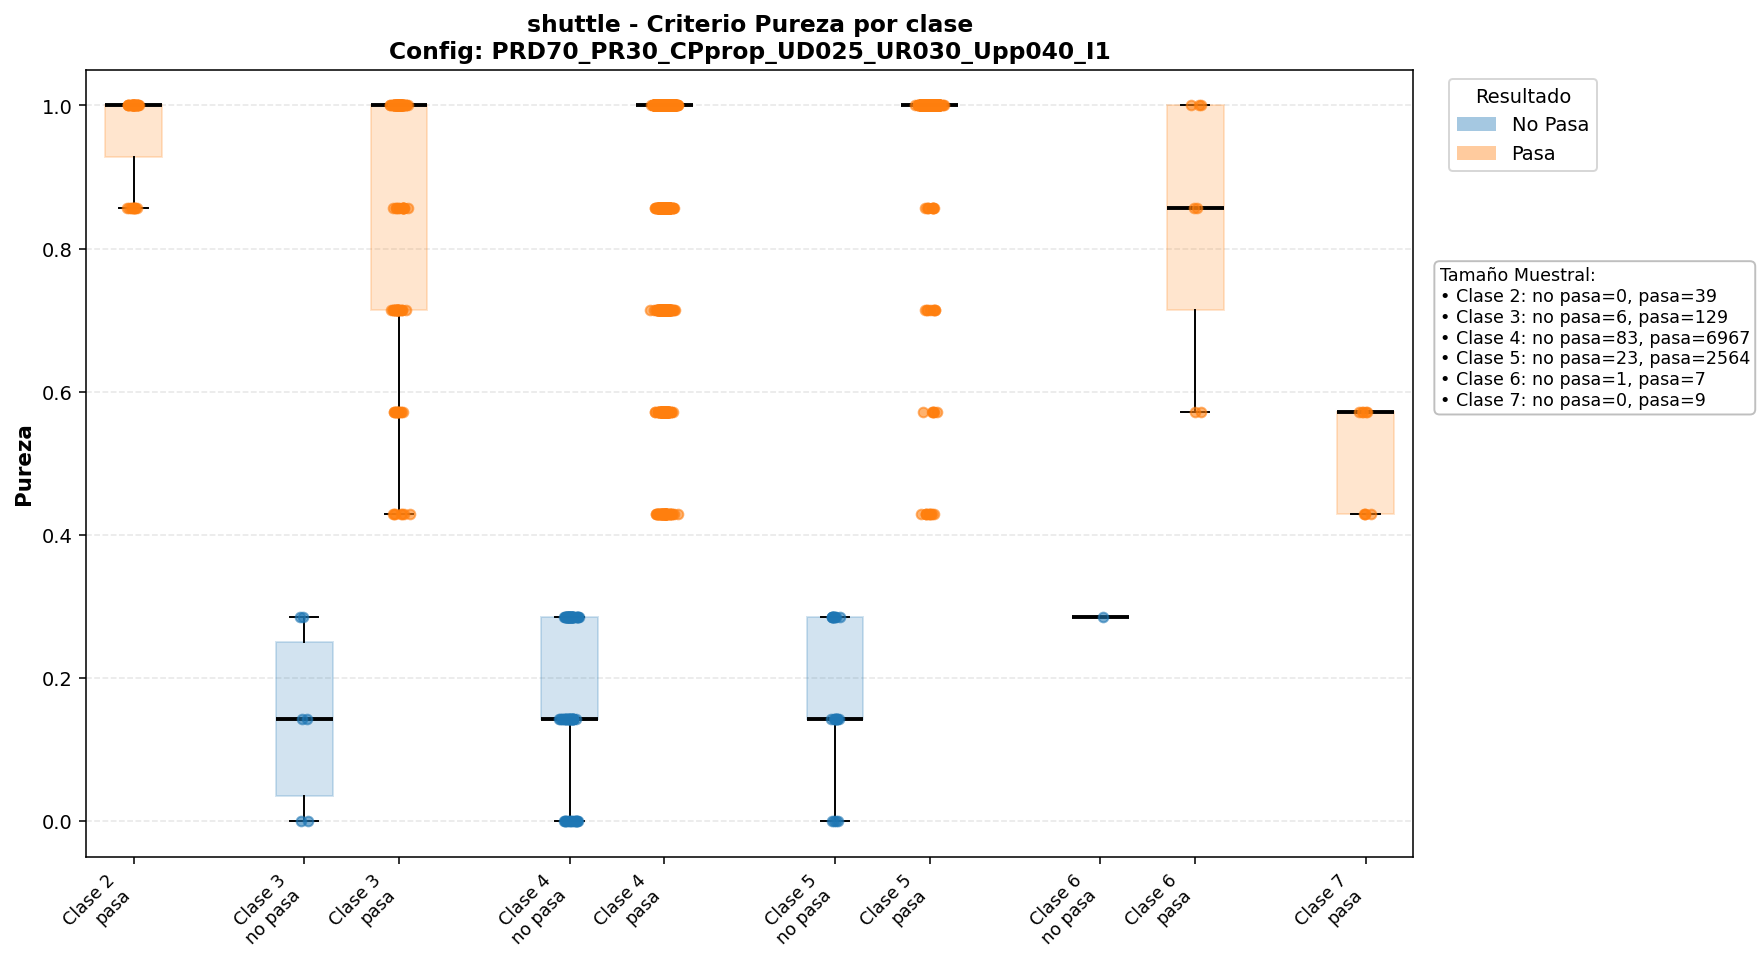
\includegraphics[width=1\textwidth]{purezas/shuttle_dotbox_Pureza.png}
    
    % El epígrafe (caption)
    \caption{Visualizacion de purezas por clase del dataset Shuttle.}
    \label{fig:mi_grafico_6}
\end{figure}

% Pureza Telco_churn todas las clases
\begin{figure}[ht]
    \centering
    % Reemplaza 'nombre_de_tu_archivo' por el nombre de tu imagen (ej. 'grafico_f1.png')
    % El [width=0.8\textwidth] escala la imagen al 80% del ancho del texto
    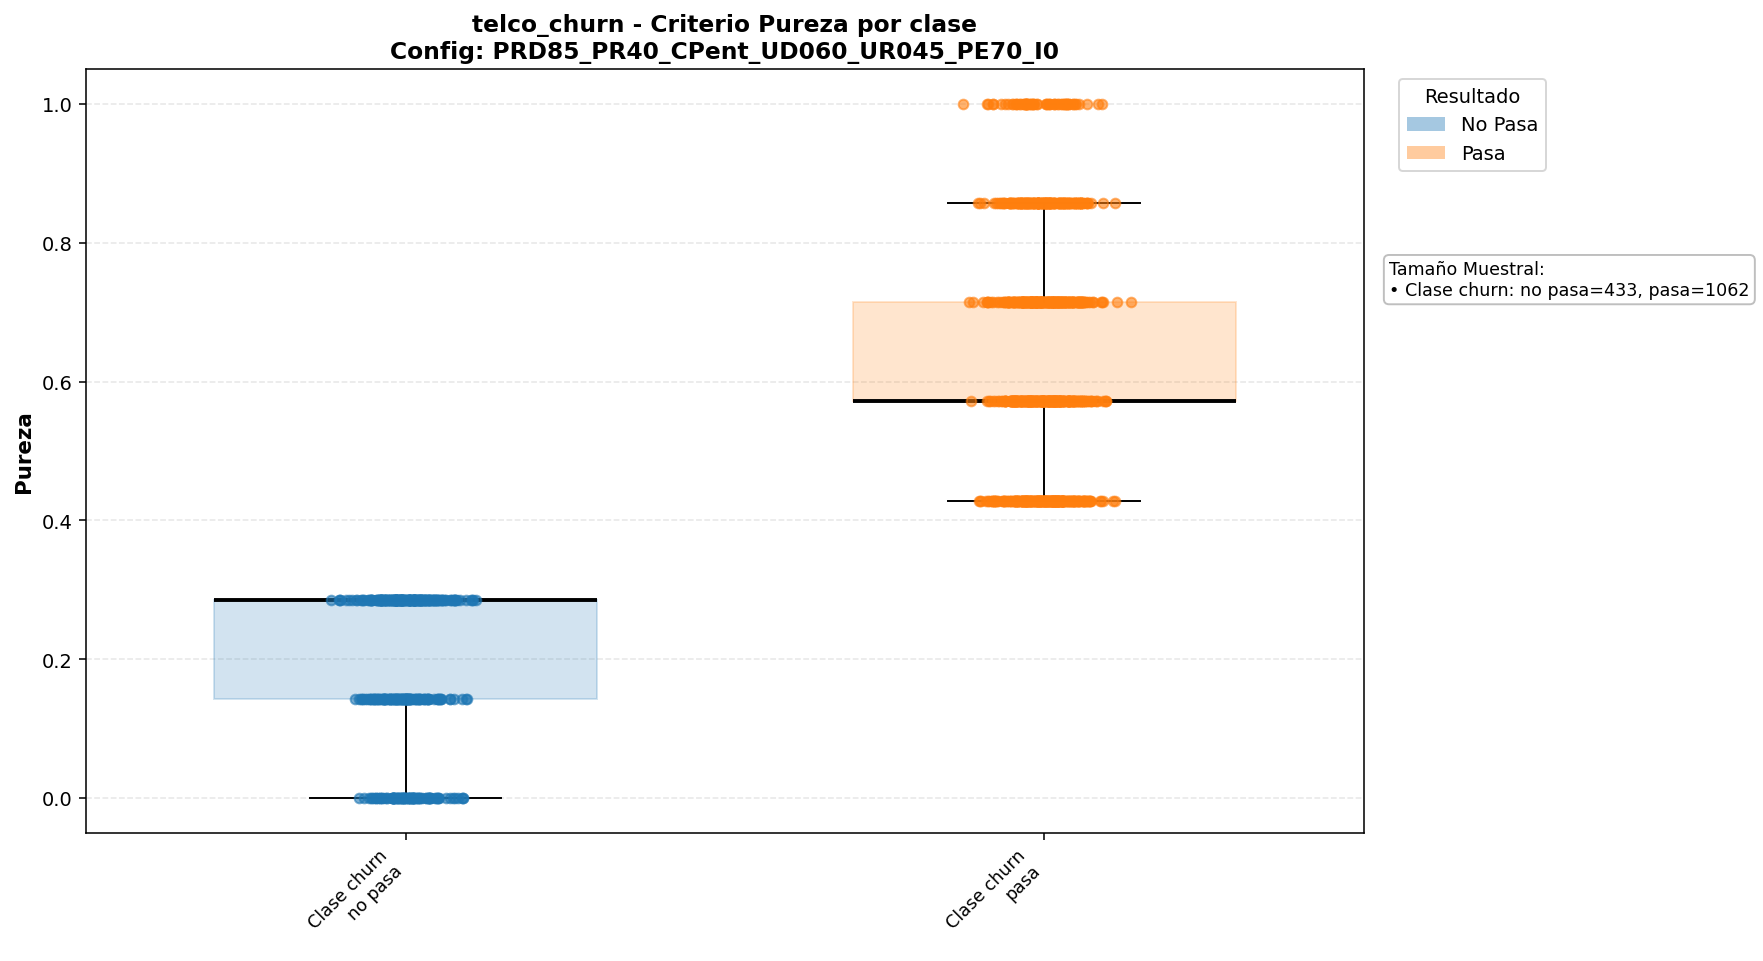
\includegraphics[width=1\textwidth]{purezas/telco_churn_dotbox_Pureza.png}
    
    % El epígrafe (caption)
    \caption{Visualizacion de purezas por clase del dataset Telco Churn. }
    \label{fig:mi_grafico_7}
\end{figure}

% Pureza US_Crime todas las clases
\begin{figure}[ht]
    \centering
    % Reemplaza 'nombre_de_tu_archivo' por el nombre de tu imagen (ej. 'grafico_f1.png')
    % El [width=0.8\textwidth] escala la imagen al 80% del ancho del texto
    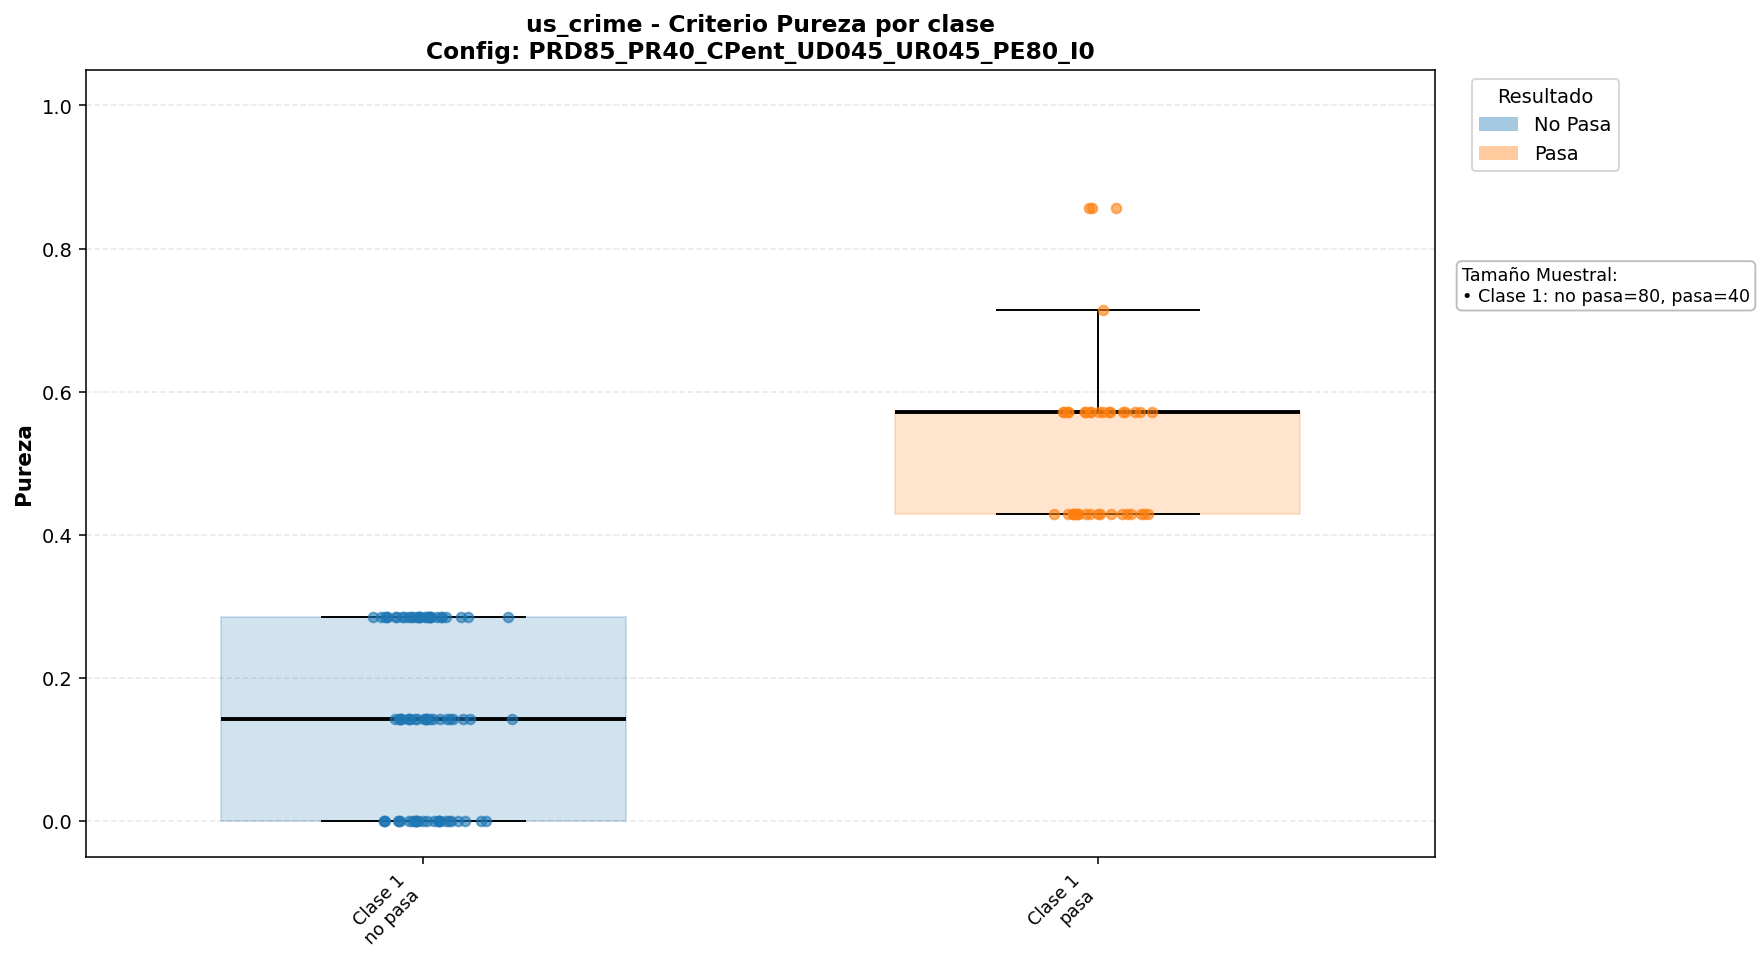
\includegraphics[width=1\textwidth]{purezas/us_crime_dotbox_Pureza.png}
    
    % El epígrafe (caption)
    \caption{Visualizacion de purezas por clase del dataset US Crime.}
    \label{fig:mi_grafico_8}
\end{figure}

% Pureza predict_faults todas las clases
\begin{figure}[ht]
    \centering
    % Reemplaza 'nombre_de_tu_archivo' por el nombre de tu imagen (ej. 'grafico_f1.png')
    % El [width=0.8\textwidth] escala la imagen al 80% del ancho del texto
    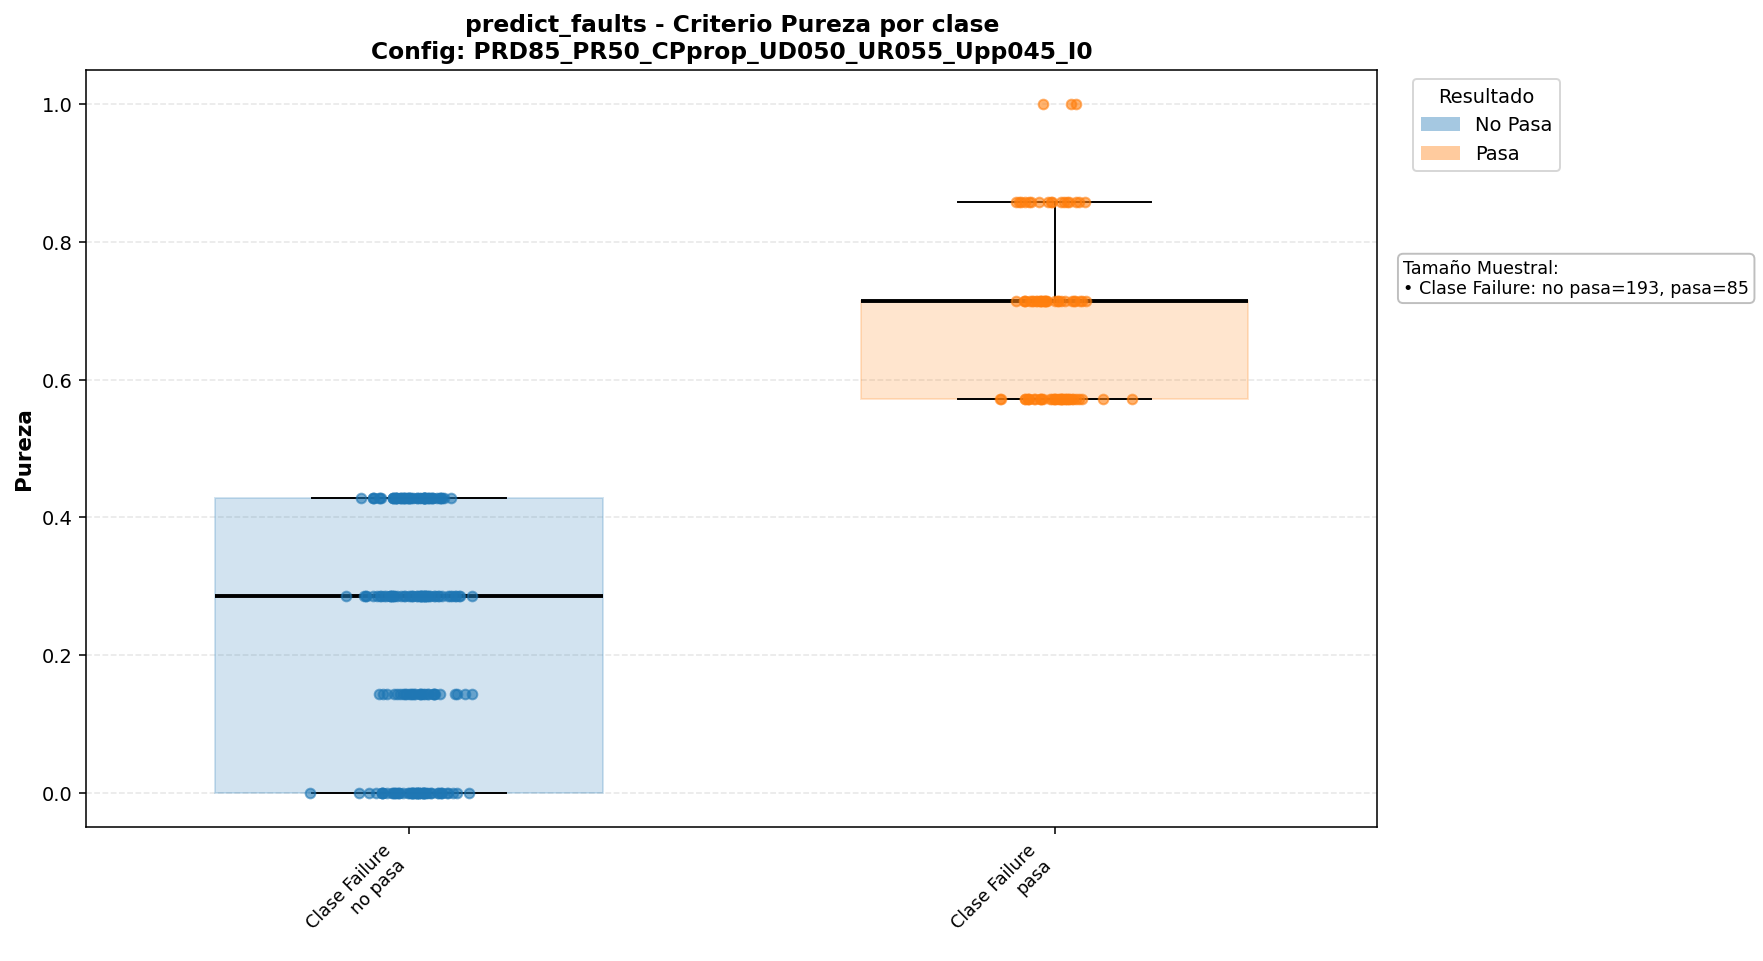
\includegraphics[width=1\textwidth]{purezas/predict_faults_dotbox_Pureza.png}
    
    % El epígrafe (caption)
    \caption{Visualizacion de purezas por clase del dataset Predict Faults.}
    \label{fig:mi_grafico_9}
\end{figure}


% RADARES COMPARATIVOS CONFIGS
\begin{figure}[ht]
    \centering
    % Reemplaza 'nombre_de_tu_archivo' por el nombre de tu imagen (ej. 'grafico_f1.png')
    % El [width=0.8\textwidth] escala la imagen al 80% del ancho del texto
    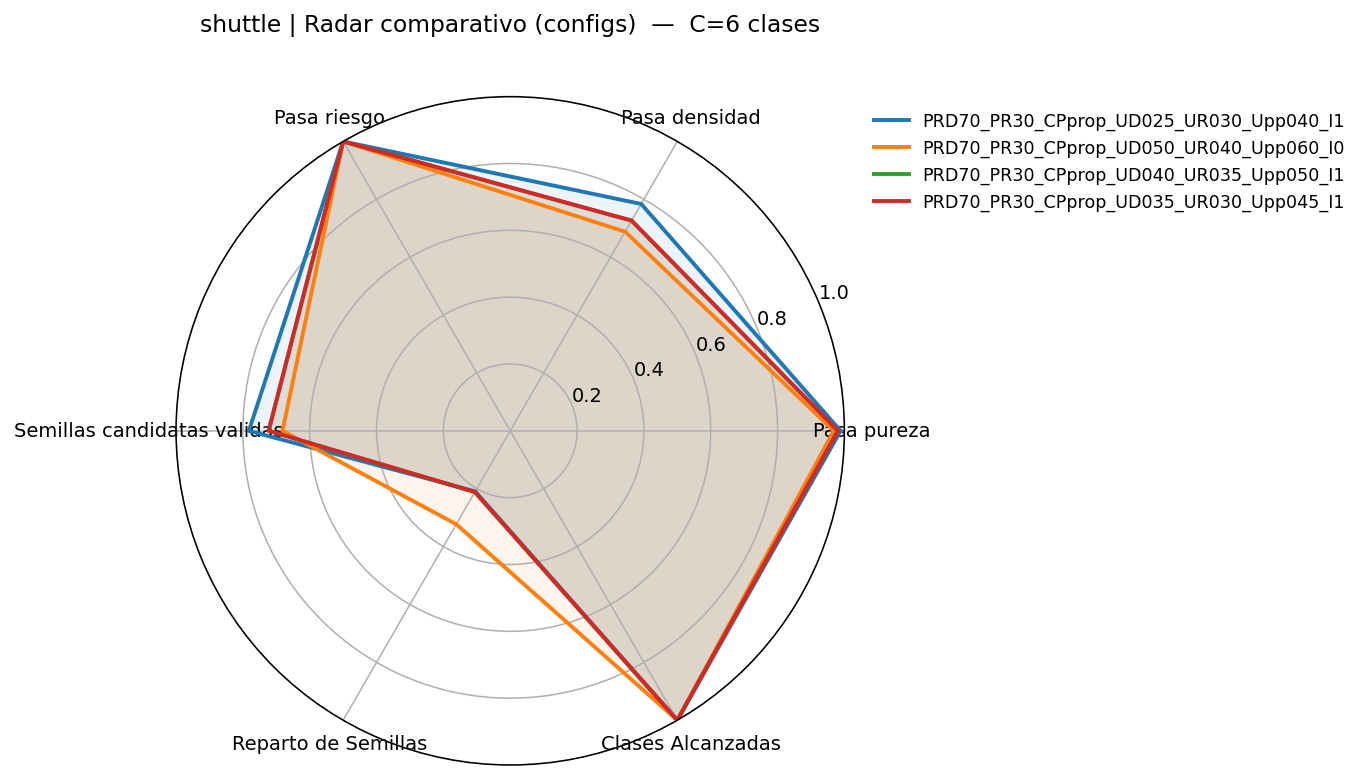
\includegraphics[width=1\textwidth]{radares/shuttle__radar_configs.png}
    
    % El epígrafe (caption)
    \caption{Radar comparativo (configs) del dataset Shuttle.}
    \label{fig:mi_grafico_1}
\end{figure}

\begin{figure}[ht]
    \centering
    % Reemplaza 'nombre_de_tu_archivo' por el nombre de tu imagen (ej. 'grafico_f1.png')
    % El [width=0.8\textwidth] escala la imagen al 80% del ancho del texto
    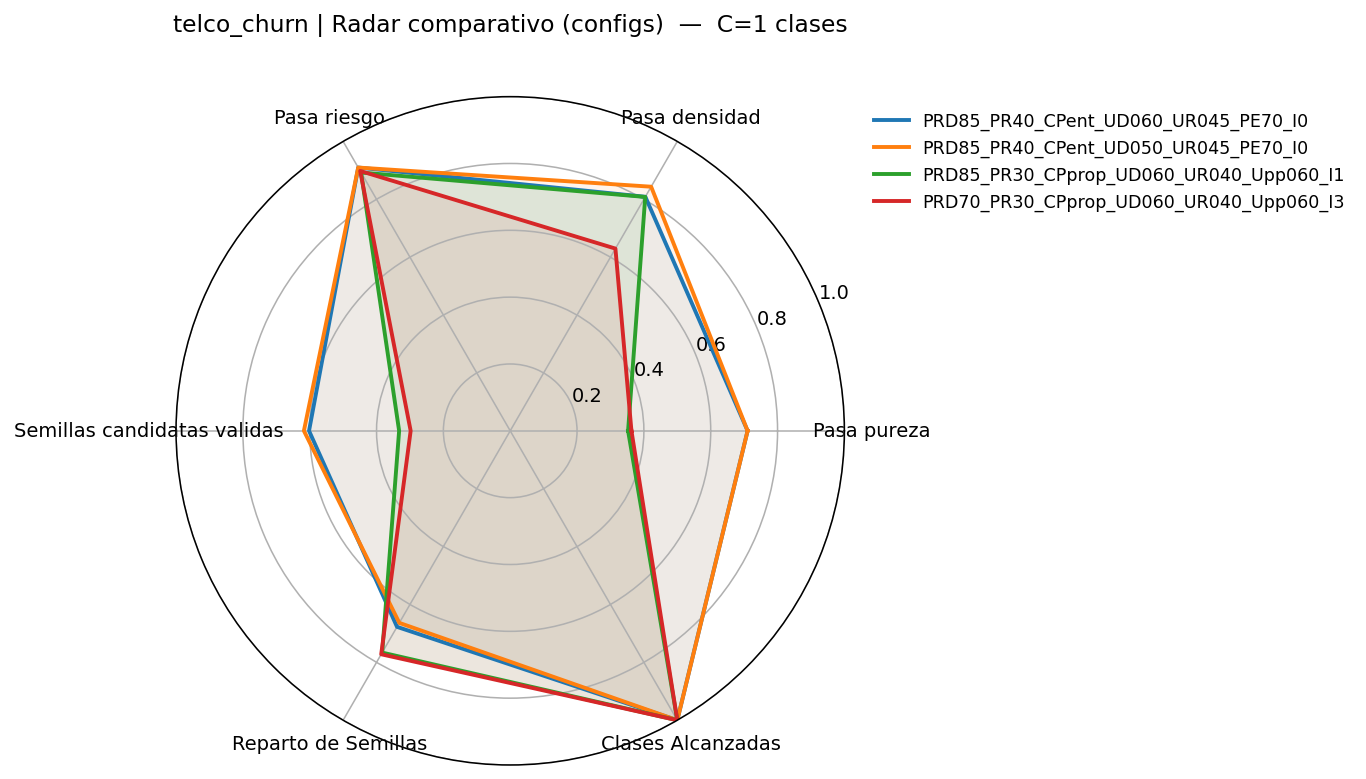
\includegraphics[width=1\textwidth]{radares/telco_churn__radar_configs.png}
    
    % El epígrafe (caption)
    \caption{Radar comparativo (configs) del dataset Telco Churn.}
    \label{fig:mi_grafico_2}
\end{figure}

\begin{figure}[ht]
    \centering
    % Reemplaza 'nombre_de_tu_archivo' por el nombre de tu imagen (ej. 'grafico_f1.png')
    % El [width=0.8\textwidth] escala la imagen al 80% del ancho del texto
    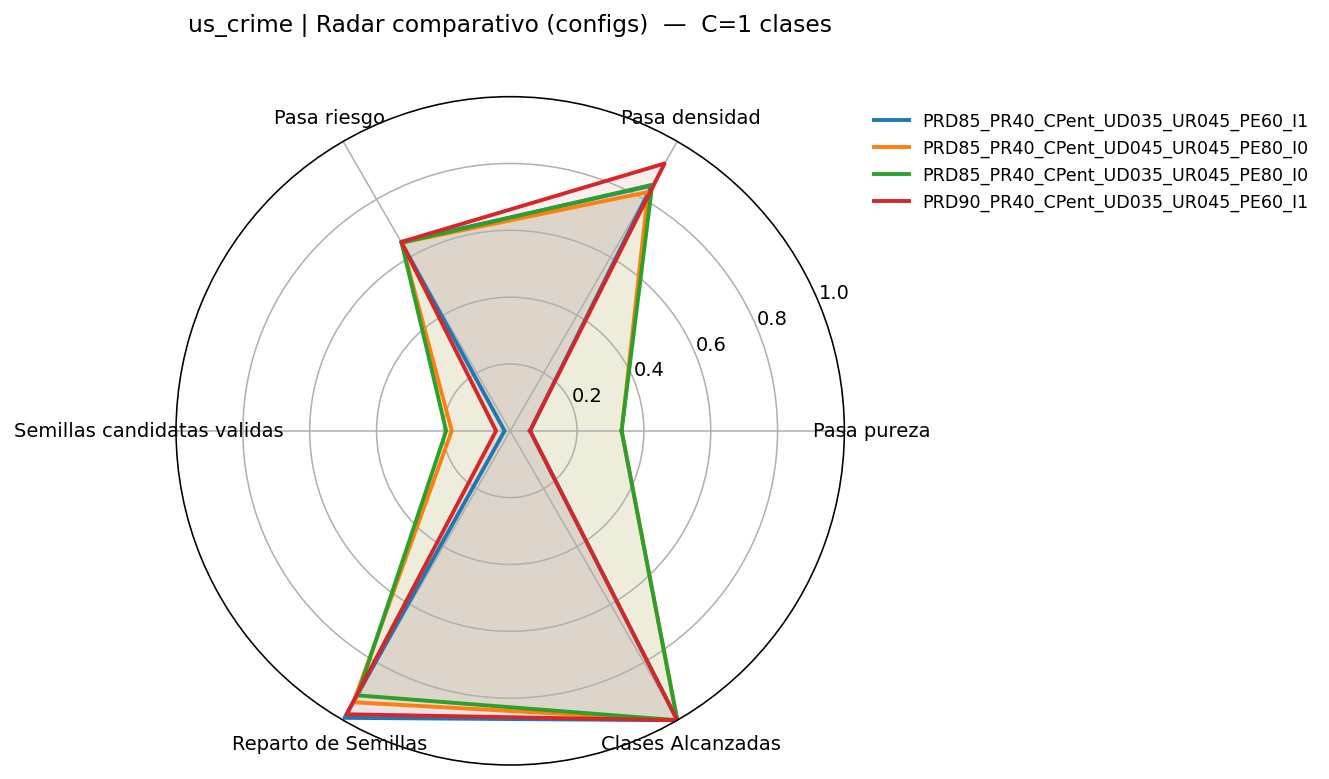
\includegraphics[width=1\textwidth]{radares/us_crime__radar_configs.png}
    
    % El epígrafe (caption)
    \caption{Radar comparativo (configs) del dataset US Crime.}
    \label{fig:mi_grafico_3}
\end{figure}

\begin{figure}[ht]
    \centering
    % Reemplaza 'nombre_de_tu_archivo' por el nombre de tu imagen (ej. 'grafico_f1.png')
    % El [width=0.8\textwidth] escala la imagen al 80% del ancho del texto
    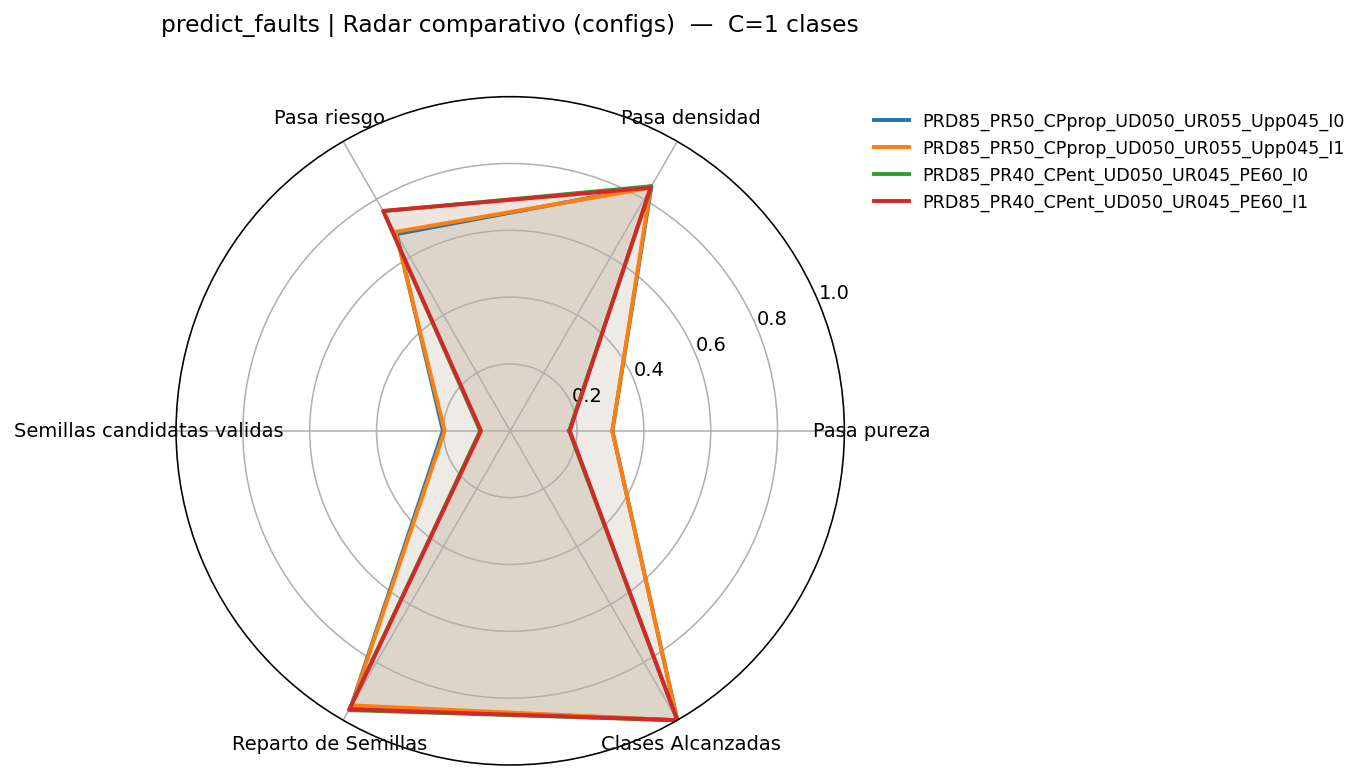
\includegraphics[width=1\textwidth]{radares/predict_faults__radar_configs.png}
    
    % El epígrafe (caption)
    \caption{Radar comparativo (configs) del dataset Predict Faults.}
    \label{fig:mi_grafico_4}
\end{figure}

\end{document}